\documentclass[11pt]{article}

% If you're new to LaTeX, here's some short tutorials:
% https://www.overleaf.com/learn/latex/Learn_LaTeX_in_30_minutes
% https://en.wikibooks.org/wiki/LaTeX/Basics

% Formatting
\usepackage[utf8]{inputenc}
\usepackage[margin=1in]{geometry}
\usepackage[titletoc,title]{appendix}
\usepackage[parfill]{parskip}

% Math
% https://www.overleaf.com/learn/latex/Mathematical_expressions
% https://en.wikibooks.org/wiki/LaTeX/Mathematics
\usepackage{amsmath,amsfonts,amssymb,mathtools}

% Images
% https://www.overleaf.com/learn/latex/Inserting_Images
% https://en.wikibooks.org/wiki/LaTeX/Floats,_Figures_and_Captions
\usepackage{graphicx,float}

% Tables
% https://www.overleaf.com/learn/latex/Tables
% https://en.wikibooks.org/wiki/LaTeX/Tables

% Algorithms
% https://www.overleaf.com/learn/latex/algorithms
% https://en.wikibooks.org/wiki/LaTeX/Algorithms
\usepackage[ruled,vlined]{algorithm2e}
\usepackage{algorithmic}

% Code syntax highlighting
% https://www.overleaf.com/learn/latex/Code_Highlighting_with_minted
%\usepackage{minted}
%\usemintedstyle{borland}

% References
% https://www.overleaf.com/learn/latex/Bibliography_management_in_LaTeX
% https://en.wikibooks.org/wiki/LaTeX/Bibliography_Management
\usepackage{biblatex}
%\addbibresource{references.bib}

% Title content
\title{Visual Data Science - Lap Part 2}
\author{Manuel Eiweck - 01633012}
\date{January 15, 2021}

\begin{document}

\maketitle

% Abstract
%\begin{abstract}
%    Add your abstract here.
%\end{abstract}

% Introduction and Overview
\section{Dataset}

I did choose a dataset containing PC games from the popular store Steam. The dataset was created around May 2019 and contains ~27.000 game entries with each one having 18 attributes.
However, the dataset is not guaranteed to be complete. In addition, it has been already cleaned from unreleased titles and non-games like software. The original data source was the official Steam API and SteamSpy a website which collects all kind of stats from steam.

\subsection{Data preparation}

As the field 'platforms','categories' and 'genres' can contain multiple values I split these columns into one column for each different value. Example: platforms has the values windows, linux and mac, after the preparation I now have 3 columns as a bit mask representing if the game supports that platform. Furthermore, 'owners' has a lower and upper bound therefore I also split that into separated columns. As our data contains a column price we add a cloumn type which is either 'Free' or 'Paid' depending on the value of price is 0 or not.

TODO: score rating
%\bigbreak
Steam Rating
https://steamdb.info/blog/steamdb-rating/

\section{Insight - generated playtime Free to Play vs Paid games}

\subsection{What is the interesting fact you found in the data?}

I wanted to compare how the total playtime of all games is split between free-to-play and paid games.\\
I found out that about ~60 percentage comes from Free to play games while 40 percentage comes from paid games. Furthermore, I also found out that there are 3 big games who generate way more playtime alone vs thousands of games together. 

\subsection{Give a brief description how you discovered the
insight.}

First I added a column 'Total Playtime'. Where Total Playtime is \\
Total Playtime $=$ average playtime $*$ owners lower bound.\\
However we have to keep in mind that the actual value of the total playtime doesn't have to be correct. Only the relation to the different games should be useful. 
Then I created different plots and percentage evaluations to discover and explore the data. 

\subsection{Choose an appropriate visualization to show the insight.}

Figure \ref{fig:insight1_1} shows a bar chart of all games. We can see that Free games generate a bit more playtime than paid games.\\ 
\begin{figure}[h]
    \centering
    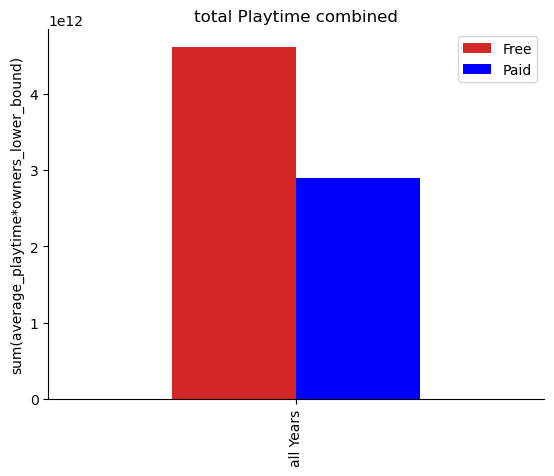
\includegraphics[width=0.5\textwidth]{graphics/insight1_graph1.png}
    \caption{Bar char of all data.}
    \label{fig:insight1_1}
\end{figure}

Figure \ref{fig:insight1_2} shows a bar chart of games separated per release year. This allows us first group our games to see if we can detect some distributions. Interesting is that games released in 2012,2013 and 2017 seems to be very popular. 
\begin{figure}
    \centering
    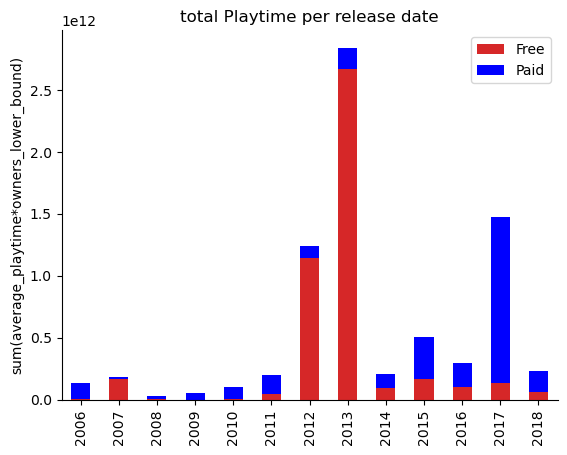
\includegraphics[width=0.5\textwidth]{graphics/insight1_graph2.png}
    \caption{Bar chart separated for release year.}
    \label{fig:insight1_2}
\end{figure}

Figure \ref{fig:insight1_3} shows a bar of the top 10 games ranked by total playtime. We can see that Dota2 released  2013, PlayerUnknown's Battlegrounds released 2017 and Counter-Strike: Global Offensive released 2012 have combined way more total playtime than the rest.\\
This explains the spikes 2012,2012 and 2017 we saw in the last graph.
\begin{figure}
    \centering
    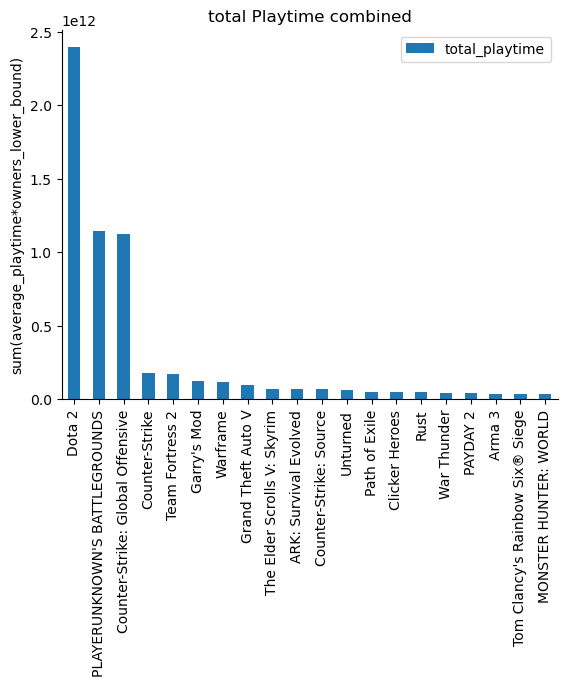
\includegraphics[width=0.5\textwidth]{graphics/insight1_graph3.png}
    \caption{Bar chart for the top 10 played games.}
    \label{fig:insight1_3}
\end{figure}

\subsection{How did you test the statistical significance of the insight?}

(i) Hypothesis:\\
1. Free to play games have more total Playtime than Paid games.\\
2. The top 3 Games are played way more than all other games together.\\
(ii)Tests:\\
As I have all the data available I decided to just use the calculated percentages\\
(iii)Check hypothesis:\\
Free to Play: 61\% vs. Paid: 39\% So we can assume that the first hypothesis is correct.\\
Playtime of top 3 games:  60\% rest: 40\% So we can assume that the second hypothesis is correct.\\

\section{Insight - Rating distribution}

\subsection{What is the interesting fact you found in the data?}

I found out that games with a more recent release date tend to have a lower rating than games with an older release date.\\

\subsection{Give a brief description how you discovered the
insight.}

As the dataset only includes the count of positive and negative reviews I used the scoring Method from "SteamDB.info" https://steamdb.info/blog/steamdb-rating/ to calculate a score from 0-1. The basic concept is to pull the score stronger towards 0.5 the less total reviews there are. So it should compensate for small  games and make them comparable to large games. 

I first created a scatter plot (see Figure \ref{fig:insight2_1}) with all games and their rating score and release date. Then I added a trend line where a falling trend was first discovered. To make sure this was not only some noise in the data I created additional plots. I decided to compare the number of released games per year from the complete dataset with released games from the top 10 percent rated games. Figure \ref{fig:insight2_2} shows the distribution of the games along the years. Additional, figure \ref{fig:insight2_3} shows the percentage of the released games being in the top 10 percent rated games of all years.  

\begin{figure}
    \centering
    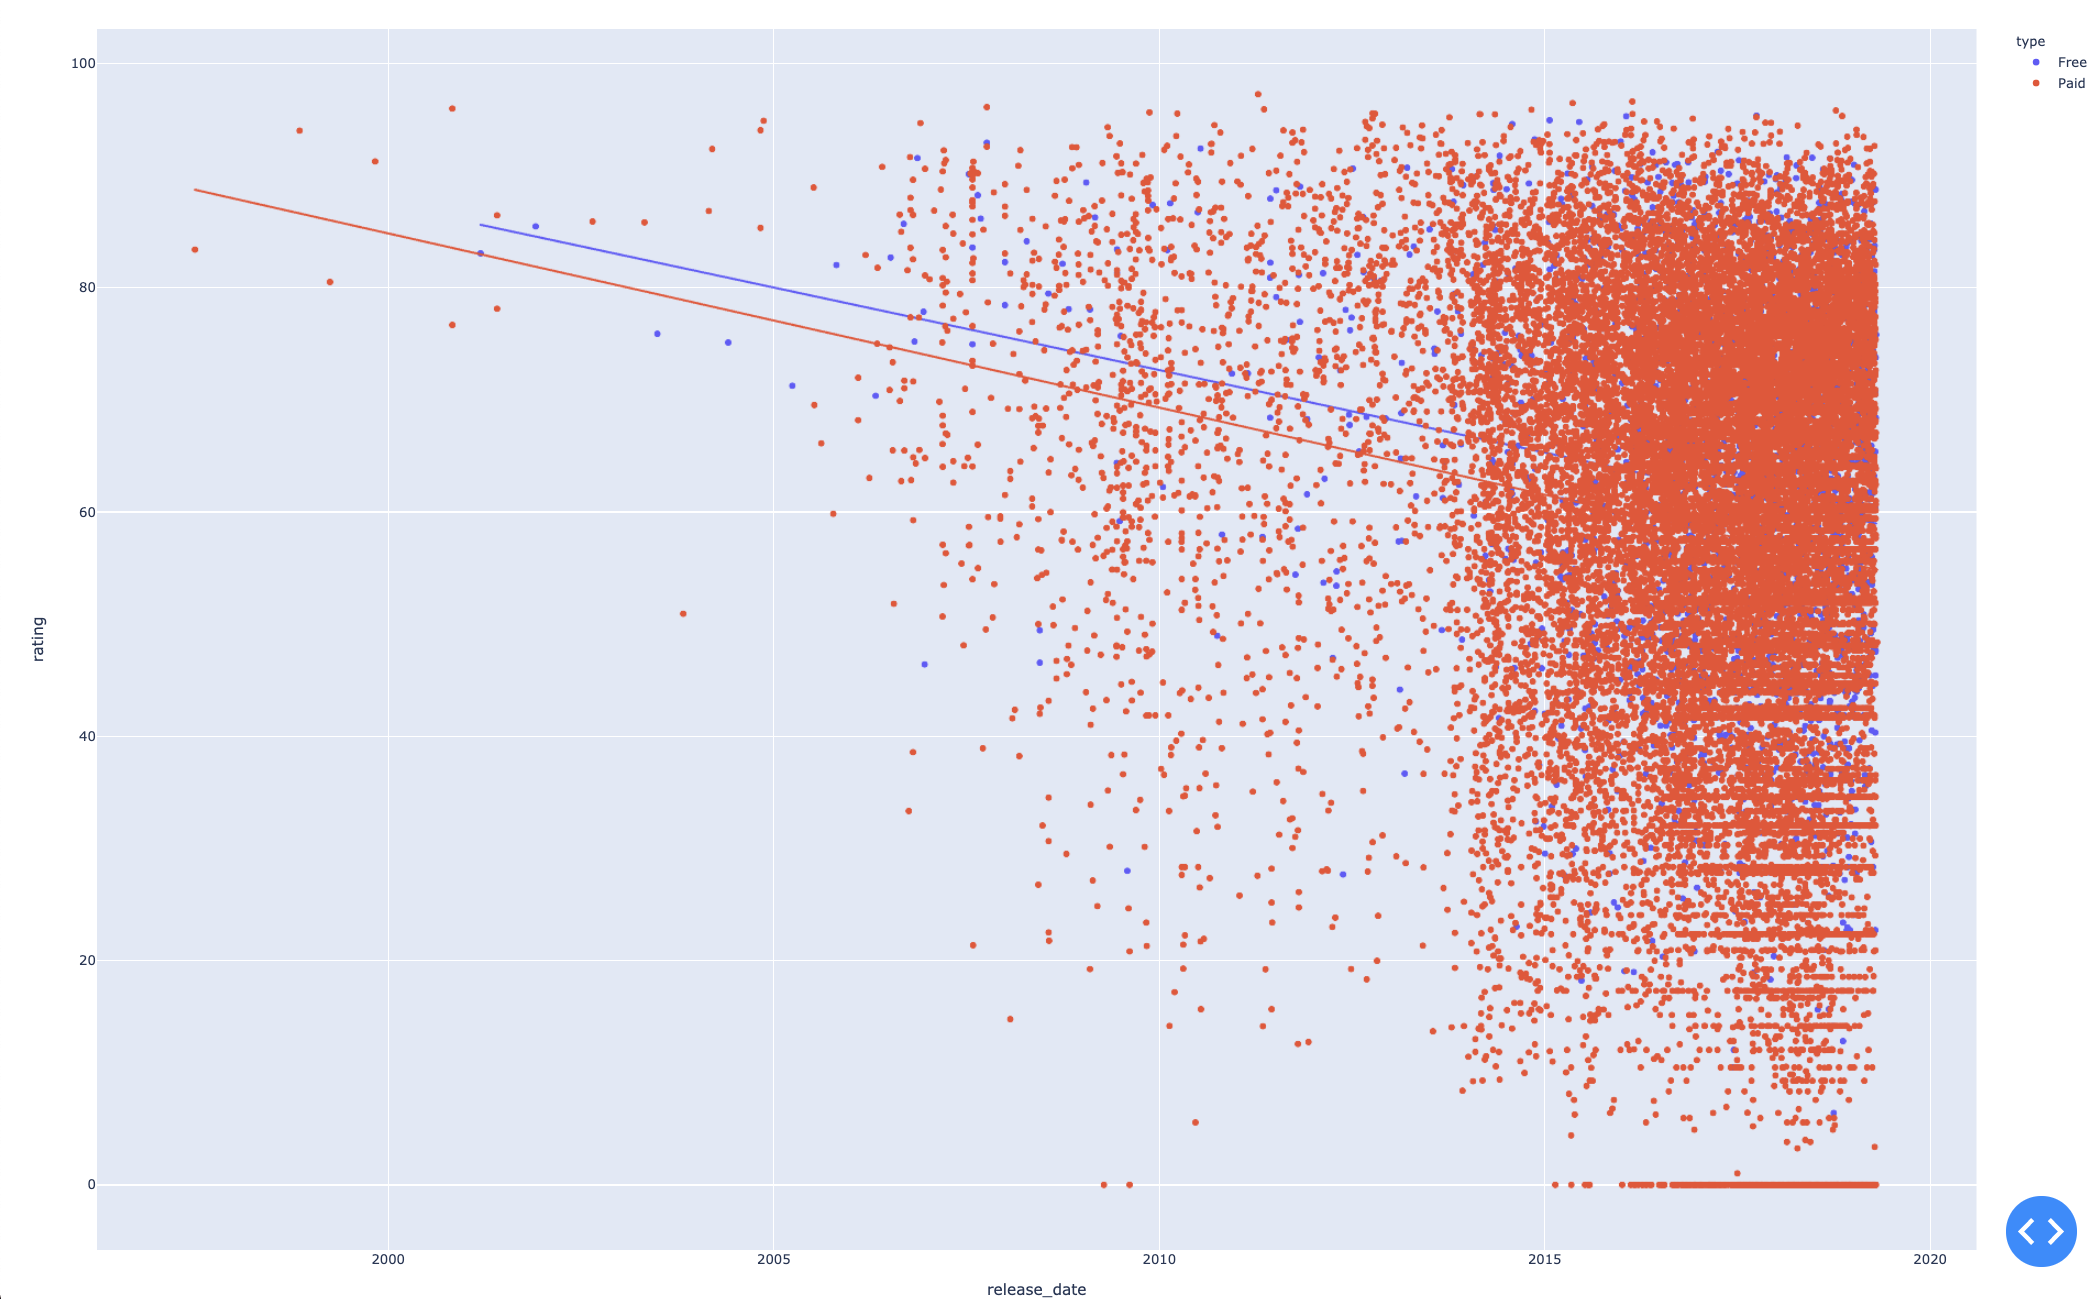
\includegraphics[width=1\textwidth]{graphics/insight2_graph1.png}
    \caption{Scatter plot for all games with rating and release date}
    \label{fig:insight2_1}
\end{figure}

\begin{figure}
    \centering
    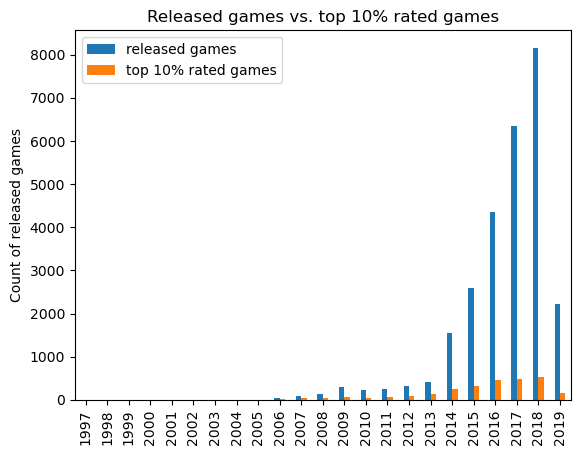
\includegraphics[width=0.5\textwidth]{graphics/insight2_graph2.png}
    \caption{Bar chart of all released games and the distribution of the top 10\% rated games.}
    \label{fig:insight2_2}
\end{figure}

\begin{figure}
    \centering
    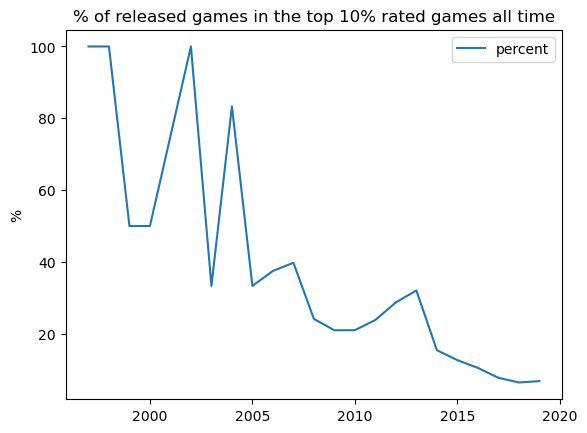
\includegraphics[width=0.5\textwidth]{graphics/insight2_graph3.png}
    \caption{Trend of released games being part of the top 10\% rated games}
    \label{fig:insight2_3}
\end{figure}

\subsection{How did you test the statistical significance of the insight?}

\section{Insight - distribution along platforms}

\subsection{What is the interesting fact you found in the data?}


\subsection{Give a brief description how you discovered the
insight.}

\subsection{Choose an appropriate visualization to show the insight.}

\subsection{How did you test the statistical significance of the insight?}

\end{document}
